\subsubsection{Strom und Ladungsträgerbewegung}

\begin{minipage}{0.5\textwidth}
\begin{itemize}
	\item linearer homogener Leiter
	\item Querschnitt A
	\item n...Dichte negativer Ladungsträger
	\item p...Dichte positiver Ladungsträger
\end{itemize}
\end{minipage} \hfill
\begin{minipage}{0.35\textwidth}
\includegraphics[width=\textwidth]{img/2_1_int}
\end{minipage}

%\begin{figure}[H]
%\includegraphics{figure1}
%\caption{\label{fig:blue_rectangle} Rectangle}
%\end{figure}

Ladungsträgerbewegung durch Querschnitt A in Zeit $\Delta t$:

$$\Delta Q = \Delta Q_p - \Delta Q_n = +e p V_p - (-e) n V_n$$

mit $V_n = A l_u$ $V_p = A l_p$

$$\Delta Q = +e p A l_p + e n A l_n$$

$$I = \frac{\Delta Q}{\Delta t} \Rightarrow I = e A (p \frac{l_p}{\Delta t} + n \frac{l_u}{\Delta t}) = e A (p v_p + n v_n)$$

Geschwindigkeit positiver Ladungsträger: $v_p = \frac{I_p}{e A p}$\\
Geschwindigkeit negativer Ladungsträger: $v_n = \frac{I_n}{e A n}$

\underbar{Beispiel:} Elektronengeschwindigkeit in Cu bei $I=1A$, $A=1mm^2$, $n_{Cu} = 8 \cdot 10^{22}cm^{-3}$

$$v_{Cu} = \frac{1 A cm^3}{1,6 \cdot 10^{-19}A s \cdot 8 \cdot 10^{22} \cdot 1mm^2} = 0,08\frac{mm}{s} = 28,8 \frac{cm}{h}$$

\subsubsection{Stromdichte}

\begin{itemize}
	\item abhängig vom Querschnitt
	\item bei linearem homogenen Leiter $S=\frac{I}{A}$
	\item allgemeiner Zusammenhang $I = \int_{(A)} \vec{s} \cdot \mathrm{d}\vec{A}$\\
		\Ra Stromdichte ist Vektor!
	\item Stromdichte und Ladungsträgergeschwindigkeit
		$$S=\frac{I}{A}=e(n \cdot v_n + p \cdot v_p)$$
	\item S ist wichtig für Strombelastbarkeit von Materialien
\end{itemize}

\subsection{Energie im Stromkreis}

Stromkreis: Ersatzschaltung für Energieumwandlungsprozesse

\begin{minipage}{0.8\textwidth}
\includegraphics[width=\textwidth]{img/2_2_int}	
\end{minipage} \hfill
\begin{minipage}{0.2\textwidth}
\Ra Stromfluss benötigt Antrieb durch Energie.
\end{minipage}

Energie W, [W] = Nm = Ws = J

\underbar{Erzeuger:}
\begin{itemize}
	\item Elemente, die $W_{and}$ in $W_{el}$ umwandeln (Batterie, Generator, Solarzelle, etc.)
	\item Bewegungsantrieb für Ladungsträger
\end{itemize}

\underbar{Verbraucher:}
\begin{itemize}
	\item Elemente, die $W_{el}$ in $W_{and}$ umwandeln (Widerstand, Motor, LED, etc.)
	\item Bewegungshemmung für Ladungsträger
\end{itemize}

\subsection{Potenzial und Spannung}

elektrisches Potenzial: potenzielle Energie im elektrischen Feld

\begin{center}
\includegraphics[width=0.7\textwidth]{img/2_3_int}
\end{center}

\begin{minipage}{0.5\textwidth}
	\vspace{1.2cm}
	$$W_1 = F \cdot h_1$$
	$$W_2 = F \cdot h_2$$
	\begin{center}
		mit $F = E \cdot Q_p$
	\end{center}
\end{minipage} \hfill
\begin{minipage}{0.5\textwidth}
	Analogie Gravitationsfeld:\\
	Kräfte zwischen Massen, potenzielle Energie
	$$W_1 = F \cdot h_1$$
	$$W_2 = F \cdot h_2$$
	\begin{center}
		mit $F = m \cdot Q_p$
	\end{center}
\end{minipage}

\fbox{$ W = E \cdot Qp $} mit r...Abstand von Ursache

Einführen eines Potenzials: \fbox{$\varphi = \frac{W}{Q}$}

$$ [\varphi] = \frac{J}{C} = \frac{Nm}{As} = \frac{Ws}{As} = V$$

\underbar{Eigenschaften:}
\begin{itemize}
	\item willkürliche Festlegung eines Bezugspotenzials $\varphi = 0$
	\item im Stromkreis höheres Potenzial am Pluspol
	\item Potenzialdifferenz:
		\begin{itemize}
			\item Ladung im elektrischen Feld wird von Punkt 1 nach Punkt 2 bewegt
			\item Energieänderung 
				$$W_{12} = W_1 - W_2 \Rightarrow \frac{W_{12}}{Q} = \frac{W_1}{Q} - \frac{W_2}{Q}$$
			\item Spannung U mit [U] = V, $U_{12} = -U_{21}$ \fbox{$= \varphi_1 - \varphi_2 = U_{12}$}
			\item Richtungssinn der Spannung: vom höheren zum niedrigeren Potenzial
		\end{itemize}
\end{itemize}

\subsubsection{Kontinuität}

Im geschlossenen Umlauf ist die Summe der Spannungen 0.

\begin{minipage}{0.5\textwidth}
	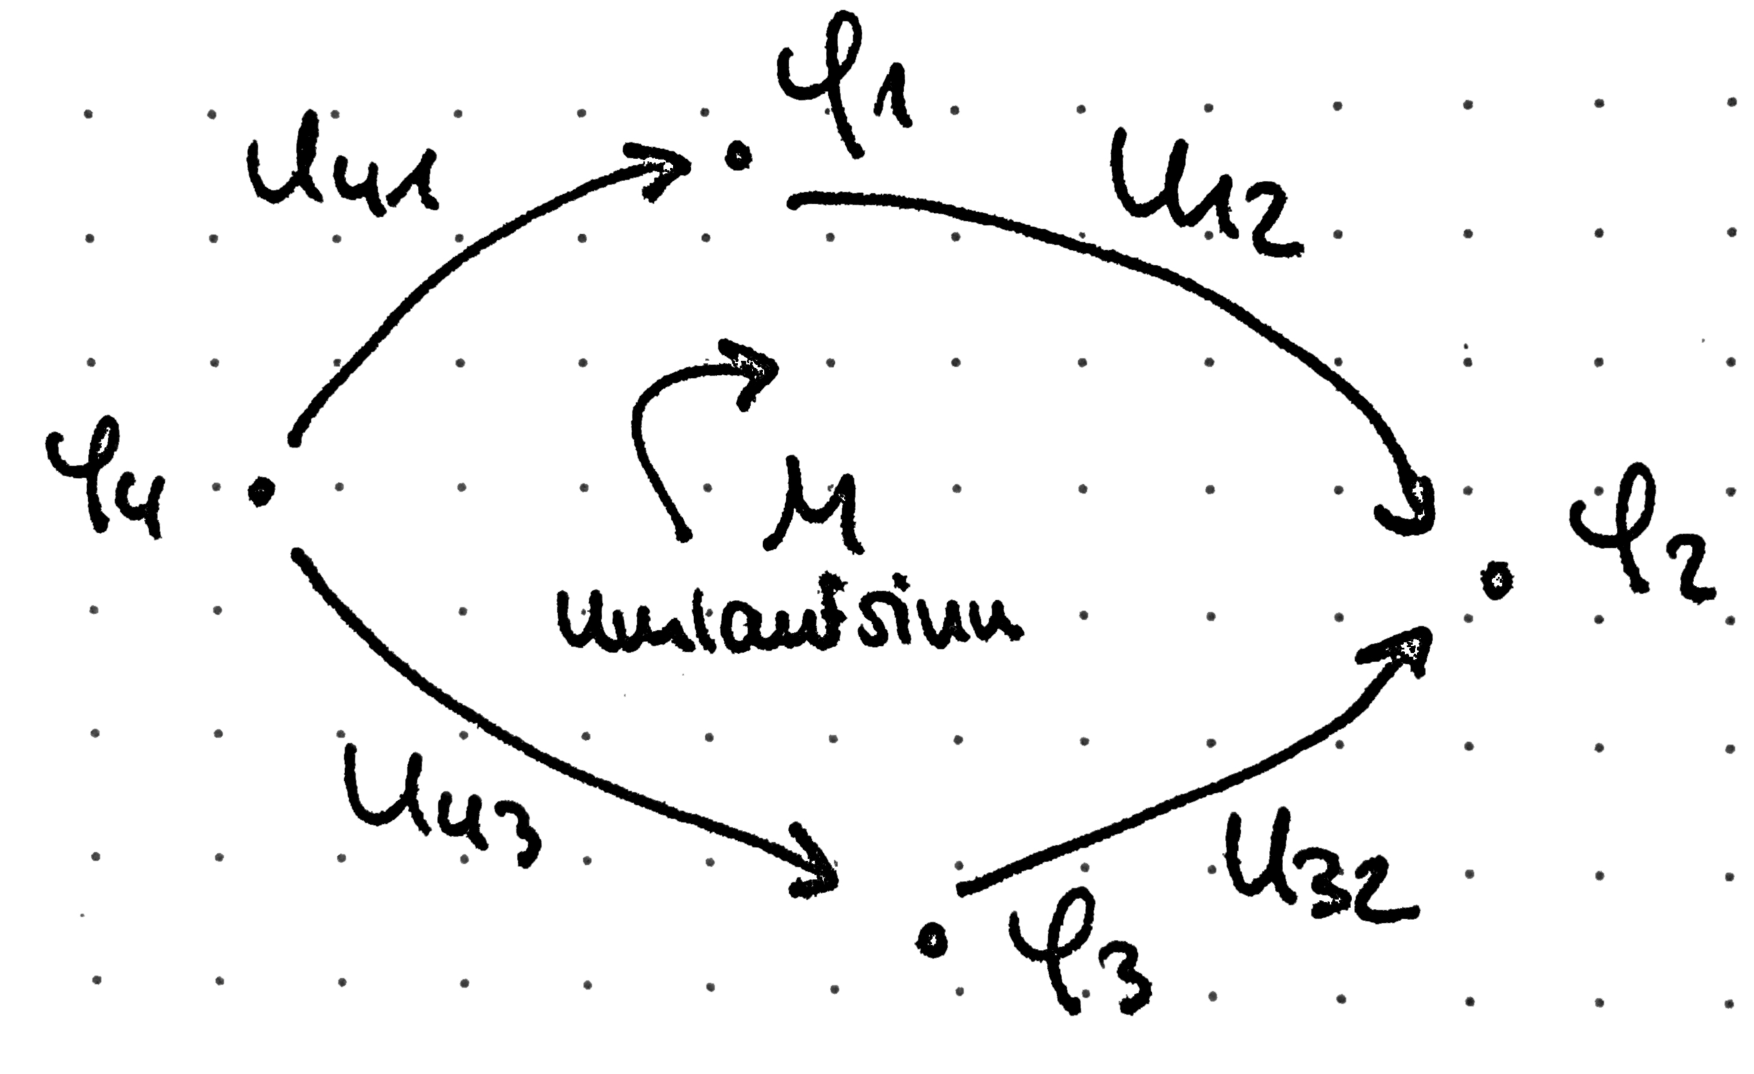
\includegraphics[width=\textwidth]{img/2_4}
\end{minipage} \hfill
\begin{minipage}{0.5\textwidth}	
	\fbox{$U_{12} - U_{32} - U_{43} + U_{41} = 0$}\\\\
	Maschensatz: $\sum u_\nu = 0$
\end{minipage}

\subsection{Elektrische Feldstärke}

bekannt:

\begin{itemize}
	\item Ladung von elektrischem Feld umgebene
	\item Kräfte zwischen Ladungen
\end{itemize}

elektrische Feldstärke \fbox{$\vec{E} = \frac{\vec{F}}{Q}$}

Vektor!\\
Richtung: vom höheren zum niedrigeren Potenzial

$$[E] = \frac{N}{As} = \frac{Nm}{Asm} = \frac{Ws}{Asm} = \frac{VA}{Am} = \frac{V}{m}$$

\subsubsection{Spannung und Feldstärke}

linearer homogener Leiter

\underbar{Gleichstrom:} Ladungsträger bewegen sich mit gleicher mittlerer Geschwindigkeit

\hspace{2cm} \Ra gleiche Kraft auf Ladungsträger

(Ladungsträger werden konstant beschleunigt und wieder abgebremst \Ra konstante mittlere Geschwindigkeit)

Energieänderung der Ladungsträger bei Bewegung von Ort 1 nach Ort 2 (Weg $l_{12}$).

$$W_{12} = F \cdot l_{12}$$
$$\frac{W_{12}}{Q} = U_{12} = \frac{F \cdot l_{12}}{Q} = E \cdot l_{12}$$
\begin{center}
\fbox{$\Rightarrow U_{12} = E \cdot l_{12}$}\\
(gilt nur für linearen, homogenen, geraden Leiter)
\end{center}

\begin{minipage}{.5\textwidth}
	\begin{itemize}
		\item linearer, homogener Leiter, $E = const.$
		\item Feldstärke E ist Maß für Potenzialgefälle
		\item E ist im Leiter nur vorhanden, wenn ein Potenzialgefälle vorhanden ist
		\item $E = 0$ im stromlosen Zustand oder bei idealen Leitern (siehe \textit{Supraleiter})
		\item E auch in Nichtleitern und Halbleitern
	\end{itemize}
\end{minipage} \hfill
\begin{minipage}{.5\textwidth}
	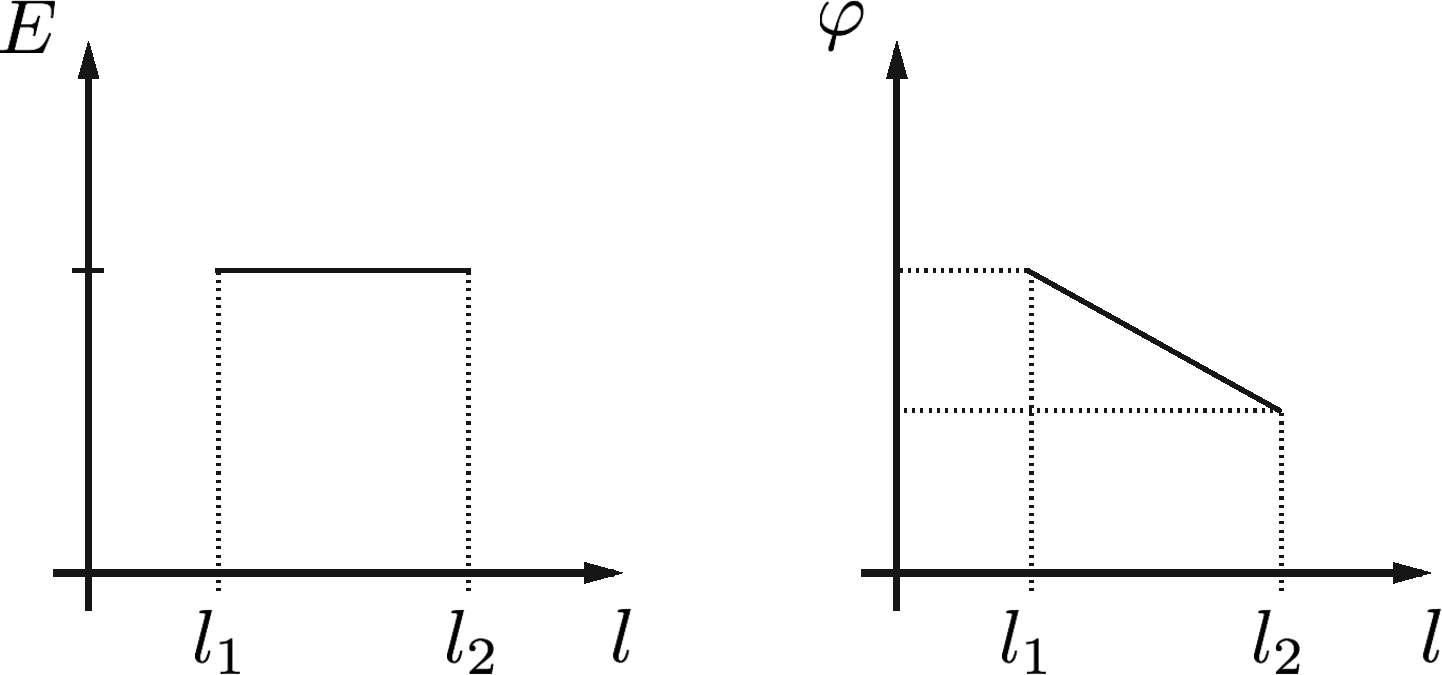
\includegraphics[width=\textwidth]{img/2_5}
\end{minipage}

\subsection{Energie, Leistung und Wirkungsgrad}

Verschieben einer Ladung Q im elektrischen Feld in der Zeit $\Delta t$.

\begin{center}
\includegraphics[width=.5\textwidth]{img/2_6_int}	
\end{center}
